\documentclass[problem]{mcs}

\begin{pcomments}
  \pcomment{CP_tiling_problem}
\end{pcomments}

\pkeywords{
 induction
 DET
 triangle
}


%%%%%%%%%%%%%%%%%%%%%%%%%%%%%%%%%%%%%%%%%%%%%%%%%%%%%%%%%%%%%%%%%%%%%
% Problem starts here
%%%%%%%%%%%%%%%%%%%%%%%%%%%%%%%%%%%%%%%%%%%%%%%%%%%%%%%%%%%%%%%%%%%%%

\begin{problem}
\emph{Divided Equilateral Triangles} (DETs) can be built up as follows:

\begin{itemize}
\item A single equilateral triangle counts as a DET whose only sub-DET is itself.

\item If $T \eqdef$ 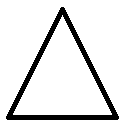
\includegraphics[width=1cm]{tiling_1} is a DET, then
  the structure built out of four copies of $T$:
\begin{center}
\begin{figure}\inbook{[h]}
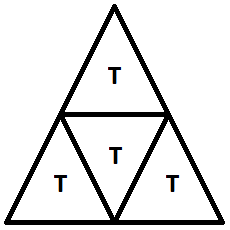
\includegraphics[width=2cm]{tiling_2}
\caption{DET from four copies of DET $T$}
\label{4DET-fig}
\end{figure}
\end{center}
is also a DET, and its sub-DETs are exactly the sub-DETS of the four copies of $T$.
\end{itemize}

\bparts

\ppart Define the \emph{length} of a DET to be the number
of sub-DETs with an edge on its base.  Prove by induction that the
total number of sub-DETS of a DET is the square of its length.

\begin{solution}
The induction hypothesis will be by strong induction on length.  The
induction hypothesis is that if the length of a DET is $n$, the total
number of sub-DETs is $n^2$.

\inductioncase{Base case} ($n = 1$) Here the only sub-DET is the
starting triangle itself, so the total number of sub-DETs is $1 = 1^2
= n^2$, proving this case.

\inductioncase{Induction step}: Suppose $T'$ is a DET with base of
length $n>1$.  Then $T'$ must consist of four copies of some DET $T$
as in Figure~\ref{4DET-fig}.  So $n=2k$ where $k$ is the length of
$T$.  Since $k<n$, we have by strong induction hypothesis that $T$ has
$k^2$ sub-DETs.  Therefore $T'$ has $4k^2$ sub-DETs.  But $4k^2 =
(2k)^2 = n^2$, proving that the number of sub-DETs of $T'$ is $n^2$ as
required.

\begin{comment}
Here is a decent false (or just misleading) proof.  Putting it here
for reference Proof by induction\\ Induction hypothesis $P(n)$: a DET
T with $n$ sub-DETs with an edge on it's base has $n^2$
sub-DETs.\\ \textbf{Base case: $n=1$} There is 1 sub-DET on the base
of T, and $1^2 = 1$ sub-DETs total.\\ \textbf{Inductive step:} Assume
by induction that $P(n)$ is true. Then suppose we have a DET with
$n+1$ sub-DETs with an edge on its base. Removing the last row of
sub-DETs gives us a DET with $n$ sub-DETs on its base, and we know by
induction that the number of sub-DETs in that portion is $n^2$.
\begin{center}
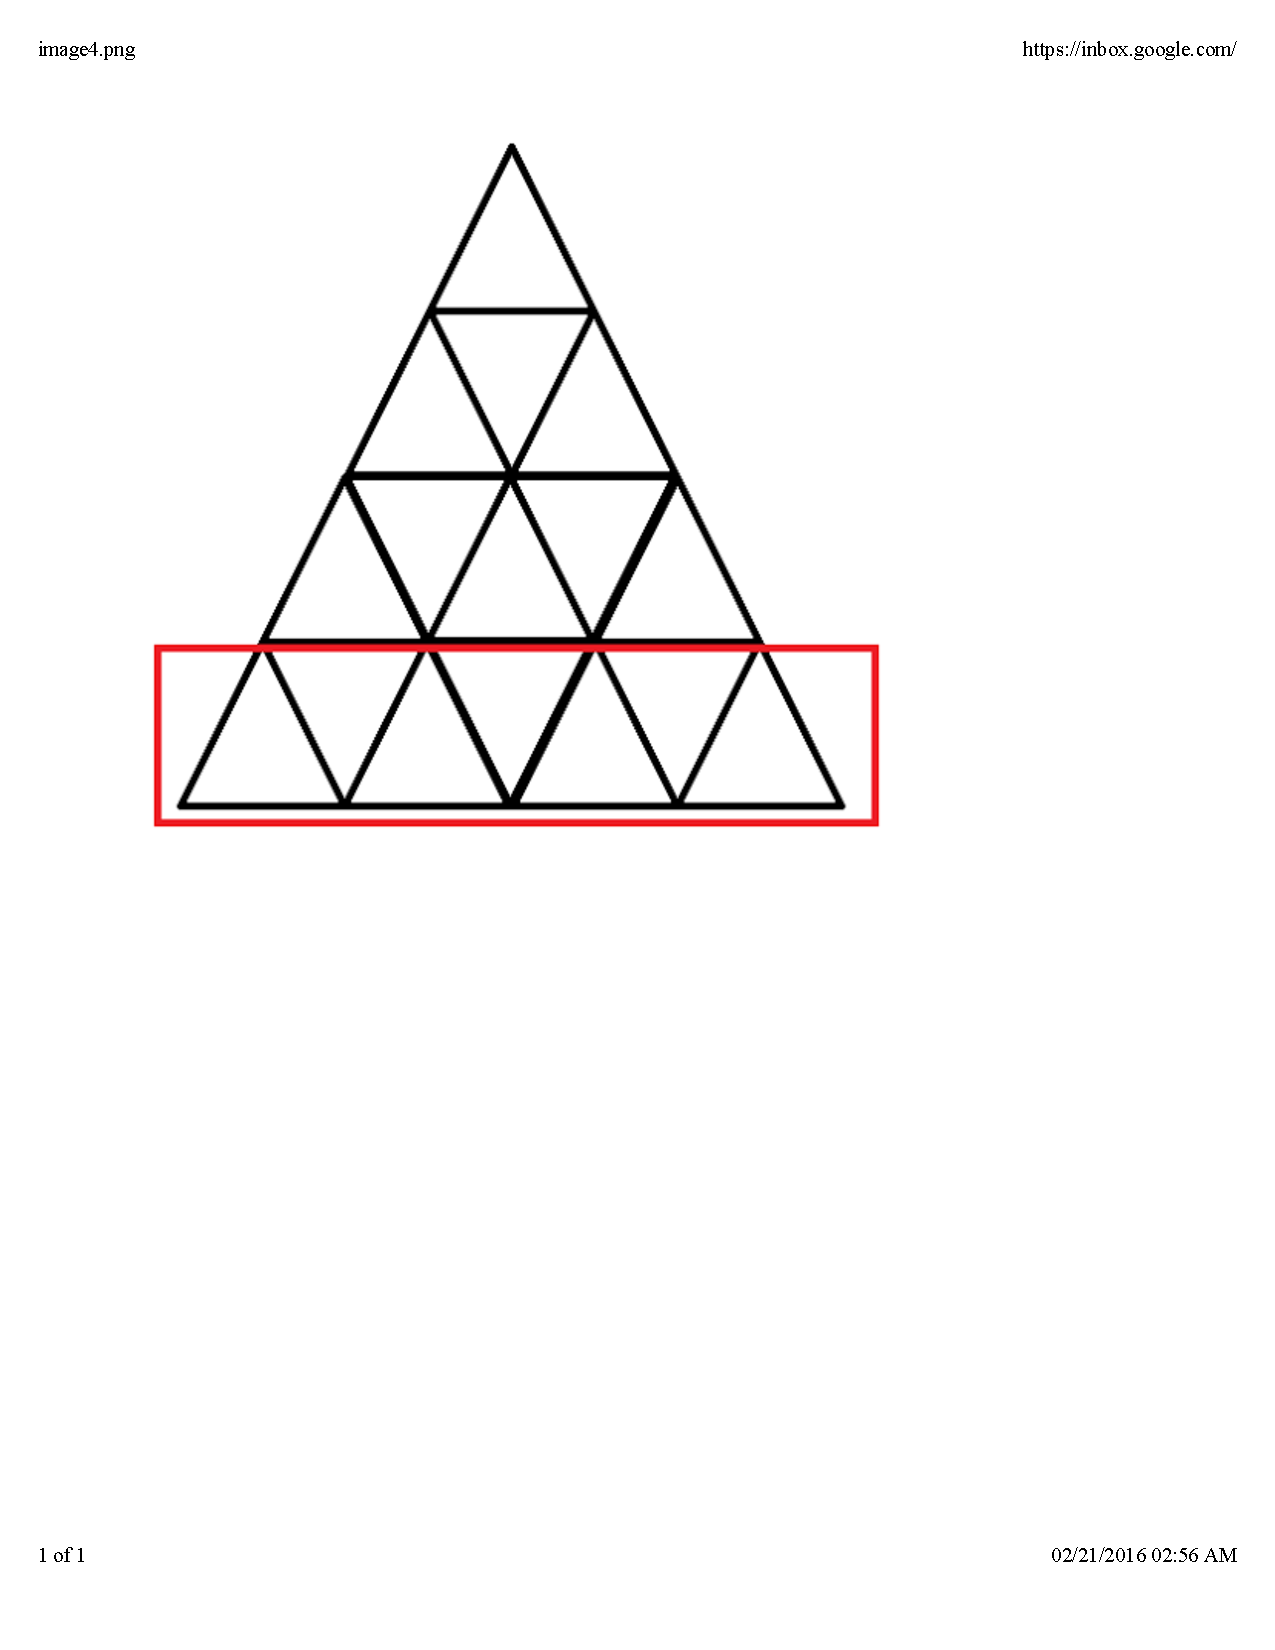
\includegraphics[width=3cm]{tiling_4}
\end{center}
How many sub-DETs did we remove? We removed the $n+1$ sub-DETs with
edges on the base, and the $n$ sub-DETs in between them. So in total
we removed $n+n+1=2n+1$ sub-DETs. And so the total number of sub-DETs
$= n^2 + 2n + 1 = (n+1)^2$. Thus, $P(n+1)$ is true. Hence, $P(n)$ is
true for all $n$.
\end{comment}

\end{solution}

\ppart Show that a DET with one of its corner sub-DETs removed can be
tiled with trapezoids built out of three sub-DETs:
\begin{center}
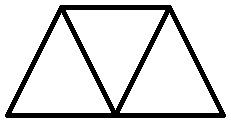
\includegraphics[width=2cm]{tiling_3}
\end{center}

\begin{solution}
Proof by induction\\
Induction hypothesis $P(n)$: a DET made out of $4n$ sub-DETs can be tiled with trapezoids build out of three sub-DETs, if one of its corner sub-DETs is removed.\\
\textbf{Base case: $n=1$} A DET built out of 4 sub-DETs. In this case, removing any corner will leave a trapezoid built out of three sub-DETs.\\
\textbf{Inductive step:} Assume by induction that each of the four DETS out of which T is built can be tiled when one their corners is removed. Then, assume (without loss of generality) that the top corner sub-DET is removed. Then, remove the right corner of 2, the top corner of 3, and the left corner of 4 (as shown in the diagram below). Now, 1, 2, 3 and 4 all have one missing corner, so by the induction hypothesis they all be tiled by trapezoids. The hole left by the middle 3 missing corners can then be tiled with a single trapezoid.
\begin{center}
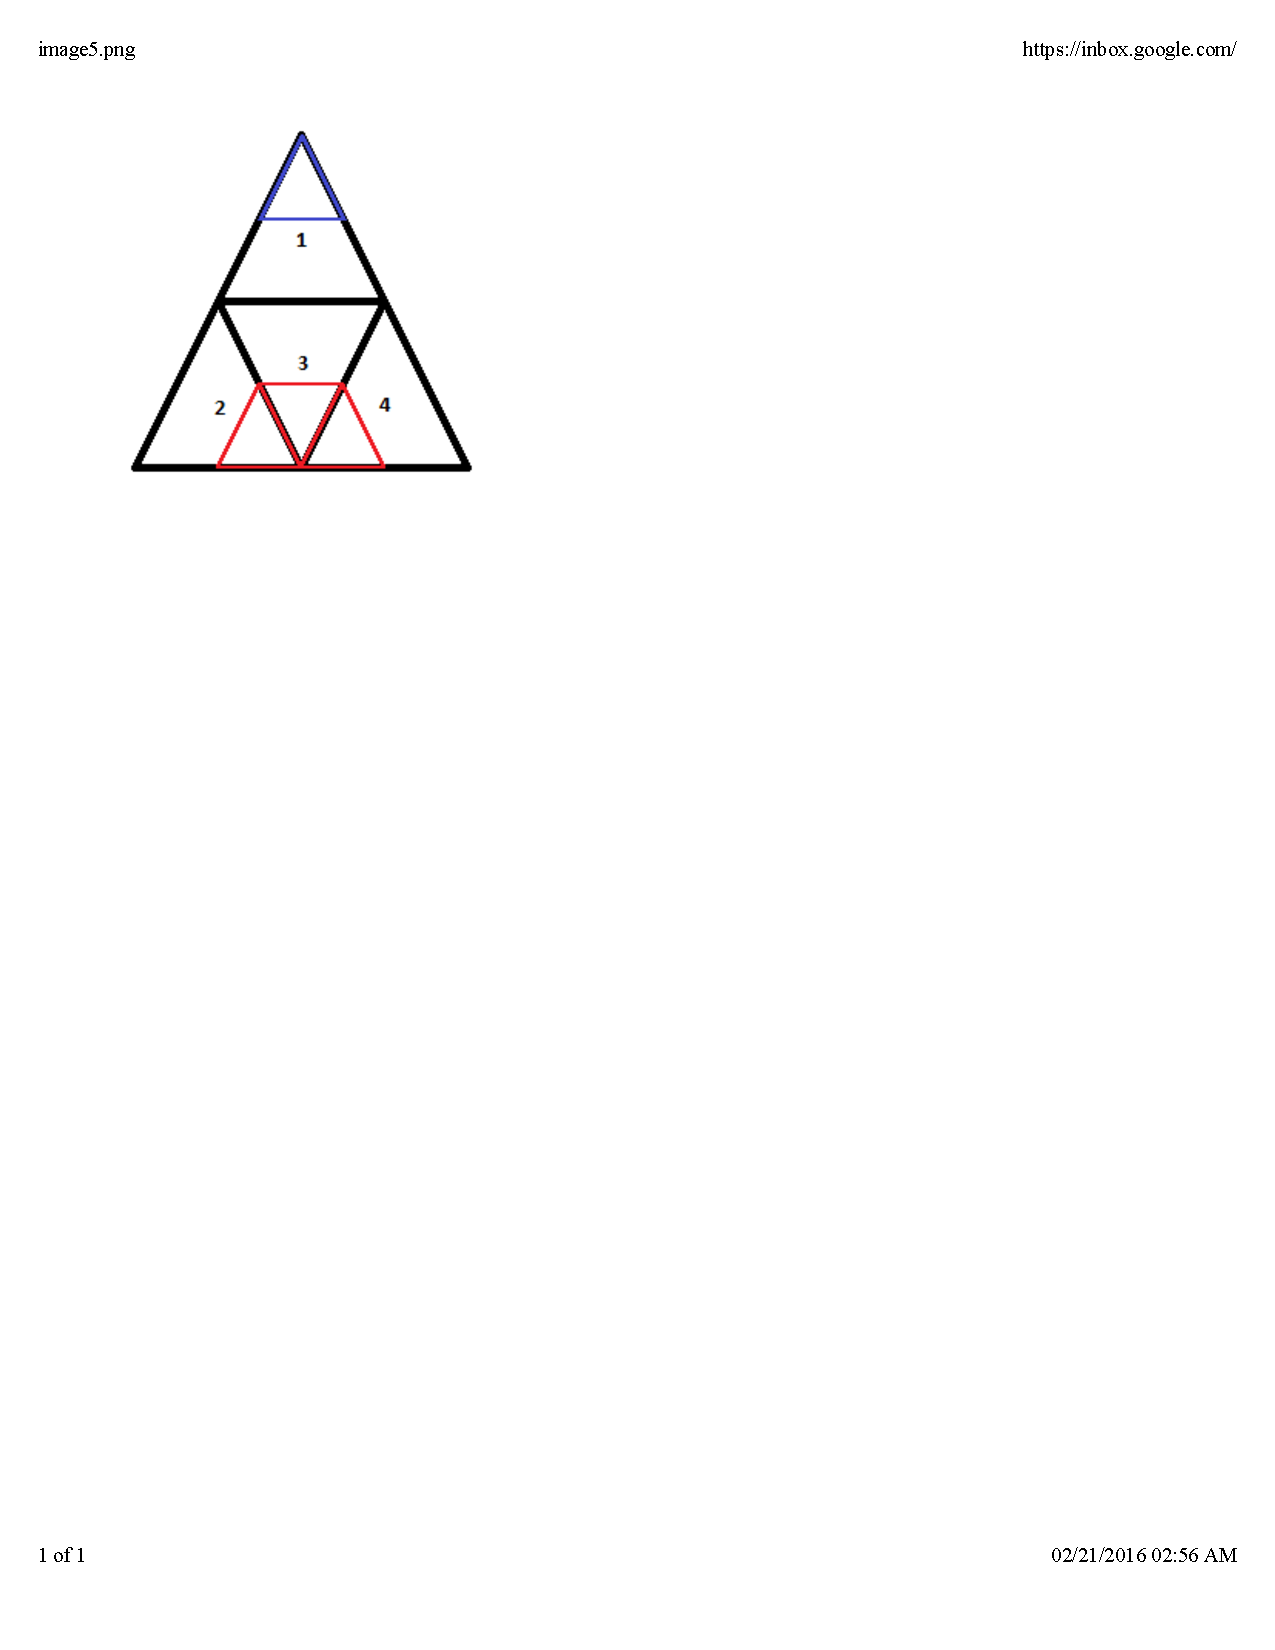
\includegraphics[width=6cm]{tiling_5}
\end{center}
\end{solution}

\eparts

\end{problem}

%%%%%%%%%%%%%%%%%%%%%%%%%%%%%%%%%%%%%%%%%%%%%%%%%%%%%%%%%%%%%%%%%%%%%
% Problem ends here
%%%%%%%%%%%%%%%%%%%%%%%%%%%%%%%%%%%%%%%%%%%%%%%%%%%%%%%%%%%%%%%%%%%%%

\endinput
